\renewcommand{\theequation}{\theenumi}
\begin{enumerate}[label=\thesection.\arabic*.,ref=\thesection.\theenumi]
\numberwithin{equation}{enumi}



































%Choose a correct answer\\
















%Choose the correct answer in each of the following:\\











%In each of the following, choose the correct answer:\\















% Choose the correct answer in each of the following:

%\item Which of the following experiments have equally likely outcomes? Explain.
% (i) A driver attempts to start a car. The car starts or does not start.\\
% (ii) A player attempts to shoot a basketball. She/he shoots or misses the shot.\\
% (iii) A trial is made to answer a true-false question. The answer is right or wrong.\\
% (iv) A baby is born. It is a boy or a girl.\\
% \item Why is tossing a coin considered to be a fair way of deciding which team should get the
%ball at the beginning of a football game?





%\item Suppose you drop a die at random on the rectangular region shown in Fig. \ref{fig:1.2.131}. What is the probability that it will land inside the circle with diameter 1m?
%\begin{figure}[!ht]
%\centering
%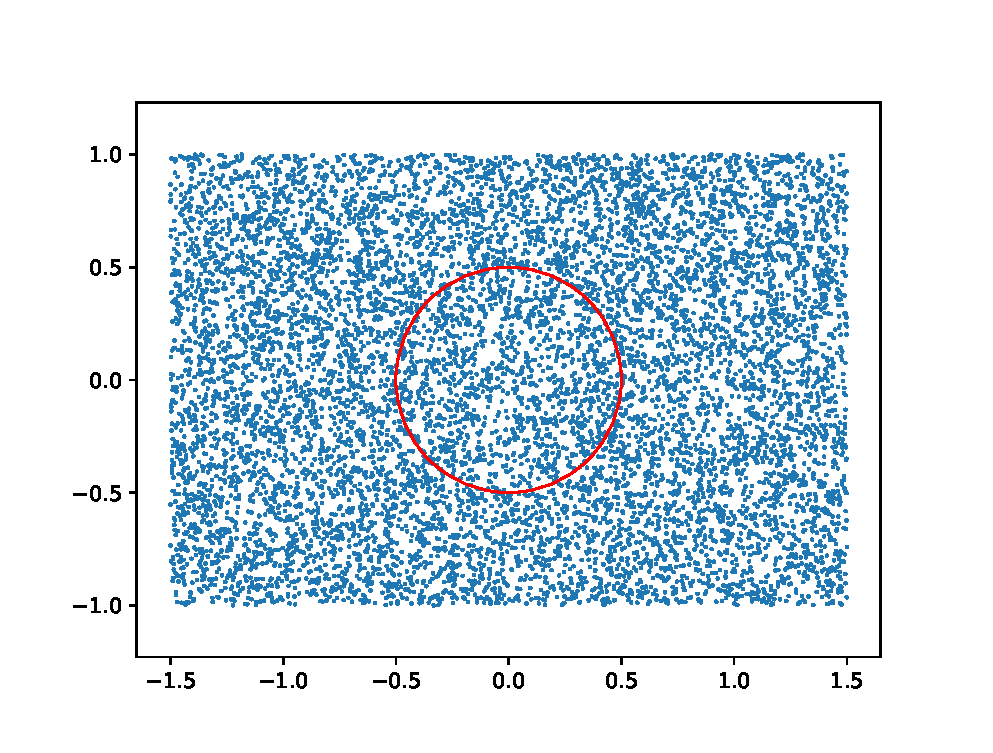
\includegraphics[width=\columnwidth]{./prob/figs/rectangle.eps}
%\caption{}
%\label{fig:1.2.131}
%\end{figure}
%\\
%\solution
%In general, the complex number $\myvec{a_1\\a_2}$ has the matrix representation
\begin{align}
\label{eq:3.4.1_Complex}
\myvec{a_1\\a_2} &= \myvec{a_1 & -a_2\\ a_2 & a_1}\myvec{1\\0}
\\
&= \vec{T}_a\myvec{1\\0}
\\
\implies \myvec{5\\-3}&=\myvec{5&3\\-3&5}\myvec{1\\0}
\end{align}
Then,
\begin{align}
\myvec{5\\-3}^3 &\triangleq\myvec{5&3\\-3&5}^3\myvec{1\\0}
\\
 &= \myvec{-10&198\\-198&-10} \myvec{1\\0}
\\
&=\myvec{-10\\-198}
\end{align}
The python code for above problem is
\begin{lstlisting}
codes/line/comp.py
\end{lstlisting}

%\begin{table}[!ht]
%\centering
%\resizebox{\columnwidth}{!}{%
%\begin{tabular}{|c|c|c|c|c|c|c|c|c|c|c|c|}
%\hline
%Event:
%'Sum on 2 dice'&2&3&4&5&6&7&8&9&10&11&12\\
%\hline
%Probability&$\frac{1}{36}$ &-&-&-&-&-& $\frac{5}{36}$ &-&-&-& $\frac{1}{36}$\\
%\hline
%\end{tabular}
%}
%\caption{}
%\label{table:1.2.133}
%\end{table}
%\solution
%In general, the complex number $\myvec{a_1\\a_2}$ has the matrix representation
\begin{align}
\label{eq:3.4.1_Complex}
\myvec{a_1\\a_2} &= \myvec{a_1 & -a_2\\ a_2 & a_1}\myvec{1\\0}
\\
&= \vec{T}_a\myvec{1\\0}
\\
\implies \myvec{5\\-3}&=\myvec{5&3\\-3&5}\myvec{1\\0}
\end{align}
Then,
\begin{align}
\myvec{5\\-3}^3 &\triangleq\myvec{5&3\\-3&5}^3\myvec{1\\0}
\\
 &= \myvec{-10&198\\-198&-10} \myvec{1\\0}
\\
&=\myvec{-10\\-198}
\end{align}
The python code for above problem is
\begin{lstlisting}
codes/line/comp.py
\end{lstlisting}


    \end{enumerate}
%\end{document}
    
